 %!TEX root = main.tex
\chapter{Models of gene regulation}

The expression of genes is tightly regulated in space and time.
One important mechanisms of gene regulation is through proteins called transcription factors that bind to specific sequences in the genome and activate or repress transcription of a nearby gene.
By combining multiple transcription factors, complicated combinatorial logic can be implemented.
Accurate regulation requires that transcription factors find their target sites reliably despite being at low concentration and the fact that the genome is wrapped around histones and coiled up in higher order chromatin structures (at least in eukaryotes).
Fig.~\ref{fig:TF_abundance} shows that in E.~coli activators (factors that increase expression) are typically present between 1 and 100 times while repressors about 10 times more abundant.
In this chapter, we will discuss simple models involving gene regulation and will draw on our previous discussions of diffusion and polymers.


\begin{figure}[tb]
	\centering
	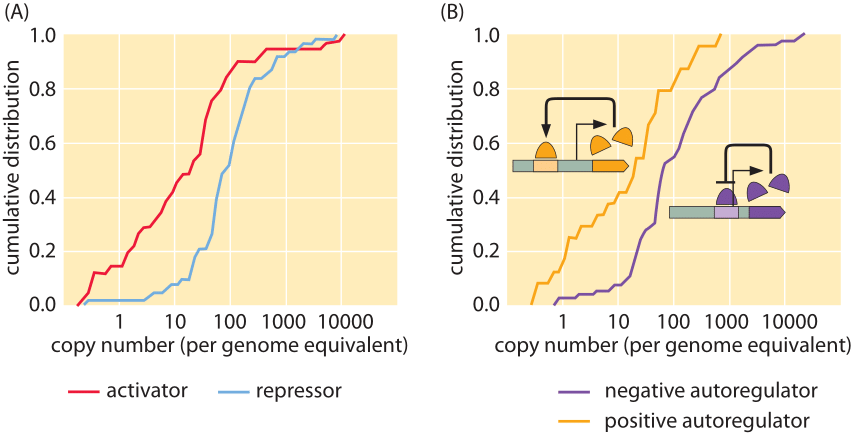
\includegraphics[width=0.9\textwidth]{figures/TFCopyNumber_bionumbers.png}
	\caption{Abundance of transcription factors in E.coli. From \href{http://book.bionumbers.org/what-are-the-copy-numbers-of-transcription-factors/}{bionumbers.org} with original data from \citep{li_quantifying_2014}. The data are shown as a cumulative distribution, that is the y-axis show the fraction of transcription factors that have an abundance below the value on the x-axis. Cumulative distributions might be a little unfamiliar to read, but have many advantages over classical histograms since they don't require a choice of binning.}
	\label{fig:TF_abundance}
\end{figure}

\section{DNA-transcription factor binding}
Given a TF is at a certain concentration and has a specific target sequence, what fraction of the time is the target sequence occupied?
This is analogous to the population of the transition state in Michaelis-Menten kinetics (page 115 in Hiller's script):
\begin{equation}
P(TF\,bound) = \frac{[X]}{K + [X]}
\end{equation}
where $[X]$ is the concentration of the TF.
The analog of the concentration of the enzyme is the DNA binding site concentration which is fixed and absorbed into $K$.
With increasing concentration, the occupation probability goes up and saturates at 1.
More often than not, transcriptional regulation is cooperative and involves multiple TFs (the same or different types).
This situation is analogous to cooperative binding of oxygen to hemoglobin: each TF individually binds to the DNA and they enhance the probability to remain bound by binding to each other.
Consider two transcription factors A and B with TF-DNA interaction free energies $\epsilon_A$ and $\epsilon_B$ and a TF-TF interaction of $J_{AB}$.
The grand partition function is then (comp.~page 78 of Hiller's script)
\begin{equation}
	\mathcal{Z} = 1 + ([A]/k_A) e^{-\epsilon_A/kT} + ([B]/k_B) e^{-\epsilon_B/kT} + ([A][B]/k_Ak_B)e^{-(\epsilon_A+\epsilon_B+J_{AB})/kT}
\end{equation}
Pulling out the concentrations, the probability that both A and B are bound is
\begin{equation}
	P_{AB} = \frac{[A][B]e^{-(\epsilon_A+\epsilon_B + J_{AB})}}{k_Ak_B +\cdots+ [A][B]e^{-(\epsilon_A+\epsilon_B+ J_{AB})}}
\end{equation}
For strongly cooperative systems, the states where only a fraction of the factors are bound don't contribute much and are often ignored.
Approximately, one has the following
\begin{equation}
	P_{AB} \approx \frac{[A][B]e^{-(\epsilon_A+\epsilon_B + J_{AB})}}{k_Ak_B + [A][B]e^{-(\epsilon_A+\epsilon_B+ J_{AB})}} = \frac{[A][B]}{K + [A][B]}
\end{equation}
where we absorbed the exponential factor into $K$.
This form of cooperative binding generalizes to $m$ copies of A and $m$ copies of $B$ as follows.
\begin{equation}
	P_{AB} \approx \frac{[A]^m[B]^n}{K + [A]^m[B]^n}
	\label{eq:hill}
\end{equation}
Here, it is important to realize that the units of $K$ change as $m$ and $n$ change, but the structure of the denominator is always the same:
$K$ is proportional to the probability of the unbound state, $[A]^m[B]^n$ is proportional to the bound state.
Curves like the ones in Eq.\ref{eq:hill} are known as Hill curves and $m$ and $n$ are Hill-coefficients (normally Hill curves consider only one species $A$ and only one coefficient $m$).
The higher the Hill-coefficient, the more cooperative and steep in the binding curve, see Fig.~\ref{fig:hill}.
Highly cooperative regulation can there yield to an almost switch like-response.

\begin{figure}[tb]
	\centering
	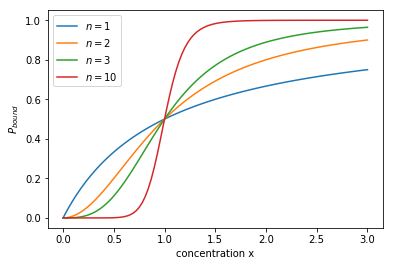
\includegraphics[width=0.48\textwidth]{Hill_curve.png}
	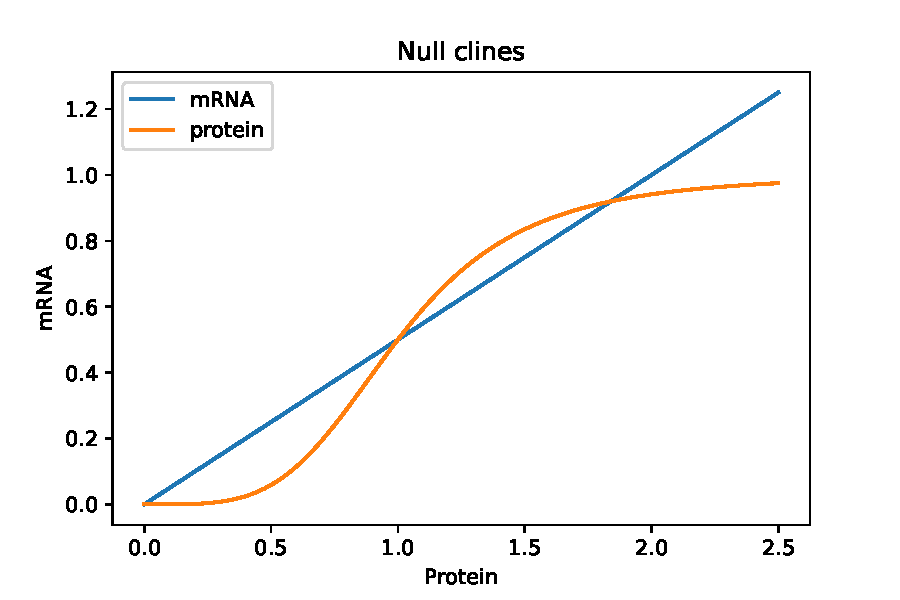
\includegraphics[width=0.48\textwidth]{null_clines.pdf}
	\caption{Left: Hill curves at different levels of cooperativity.
			Right: Null clines of the simple auto-activator system in Eqs.\ref{eq:act_mRNA} and \ref{eq:act_protein}. Units of time and concentrations are chosen such that $\alpha=\beta=1=K=1$, $n=4$, $\gamma=2, \delta=1$.}
	\label{fig:hill}
	\label{fig:null_clines}
\end{figure}


\section{Simple genetic circuits}
Which genes are transcribed at which rate at a given time is a function of the concentration of regulatory proteins, RNA polymerase, epigenetic modifications etc. -- essentially a function of the state of the cell.
To study gene expression using computational models, we will typically try to isolate the most important factors into a simple model and describe their dynamics by a system of differential equations:
\begin{eqnarray}
	\frac{d x_1}{dt} &=& f_1(x_1, x_2, \ldots, x_n, t) \\
	\frac{d x_2}{dt} &=& f_2(x_1, x_2, \ldots, x_n, t) \\
	\vdots & = & \vdots \\
	\frac{d x_n}{dt} &=& f_n(x_1, x_2, \ldots, x_n, t)
\end{eqnarray}
Here the functions $f_i(x_1,\ldots, x_n,t)$ describe how rapidly quantity $i$ is produced given the state of the cell.
This function could depend explicitly on time, for example because of daily rhythms.
Such computational models of gene expressions fall into the domain of dynamical systems.
A very good and accessible introduction to dynamical systems is the book by Steven Strogatz \citep{strogatz_nonlinear_2014}.

The simplest dynamical systems are one-dimensional and of the form
\begin{equation}
	\frac{dx}{dt} = f(x)
\end{equation}
In the case of gene expression modeling, the function $f(x)$ typically consists of a production term and a degradation term, for example like the following:
\begin{equation}
	\frac{dx}{dt} = \alpha - \beta x
\end{equation}
In this case, $x$ is produced at constant rate $\alpha$ and decays with rate $\beta$.
The concentration $x$ is going to increase whenever $\alpha > \beta x$ and decrease when $\alpha <\beta x$.
The system has hence a fixed point $\bar{x} = \alpha/\beta$.

\subsection*{Self activation:}
The simplest genetic circuits are genes that regulate their own expression.
We will first consider a gene $x$ whose transcription is regulated by its own product protein $X$.
To keep the notation simple, lets denote the mRNA concentration by $x$ and that of the protein by $X$.
mRNA is produced whenever the promoter is occupied by $n$ copies of protein $X$ and decays in a linear fashion.
\begin{equation}
\label{eq:act_mRNA}
	\frac{dx_1}{dt} = \alpha\frac{x_2^n}{K+x_2^n} - \beta x_1
\end{equation}
The parameters $\alpha$ and $\beta$ are the transcription rate and mRNA decay rates, respectively.
The mRNA is then translated to proteins such that the protein concentration evolves as
\begin{equation}
\label{eq:act_protein}
	\frac{dx_2}{dt} = \gamma x_1 - \delta x_2
\end{equation}
Here, $\gamma$ is the translation rate (the amount of protein produced by mRNA per unit of time) and $\delta$ is the degradation rate.

To a qualitative idea of the behavior of the behavior of the system, it is useful to graph the lines at which $\frac{dx_1}{dt}=\frac{dx_1}{dt}=0$.
For Eqs.\ref{eq:act_mRNA} and \ref{eq:act_protein} this results in $x_1=\delta/\gamma x_2$ and $x_1 = \frac{\alpha}{\beta}\frac{x_2^n}{K+x_2^n}$.
These lines are known as null clines are shown in Fig.~\ref{fig:null_clines}B.
Whenever the null-clines intersect, the system is at a fixed point, that is a point where the concentrations don't change.
Some of these fixed points are stable and other unstable.
A stable fixed point ``attracts'' solutions in its neighborhood, and trajectories in the vicinity of an unstable fixed point move away from the fixed point.

In the case shown in Fig.~\ref{fig:null_clines}B, there are two stable fixed points separated by one unstable fixed point.
Such systems are called bistable.
Each of the stable fixed point has a ``basin of attraction''.
Any simulation with initial condition in the basin of attraction of one fixed point will flow towards that fixed point.
Simulations of this case are shown in Fig.~\ref{fig:bistable}.

\begin{figure}[tb]
	\centering
	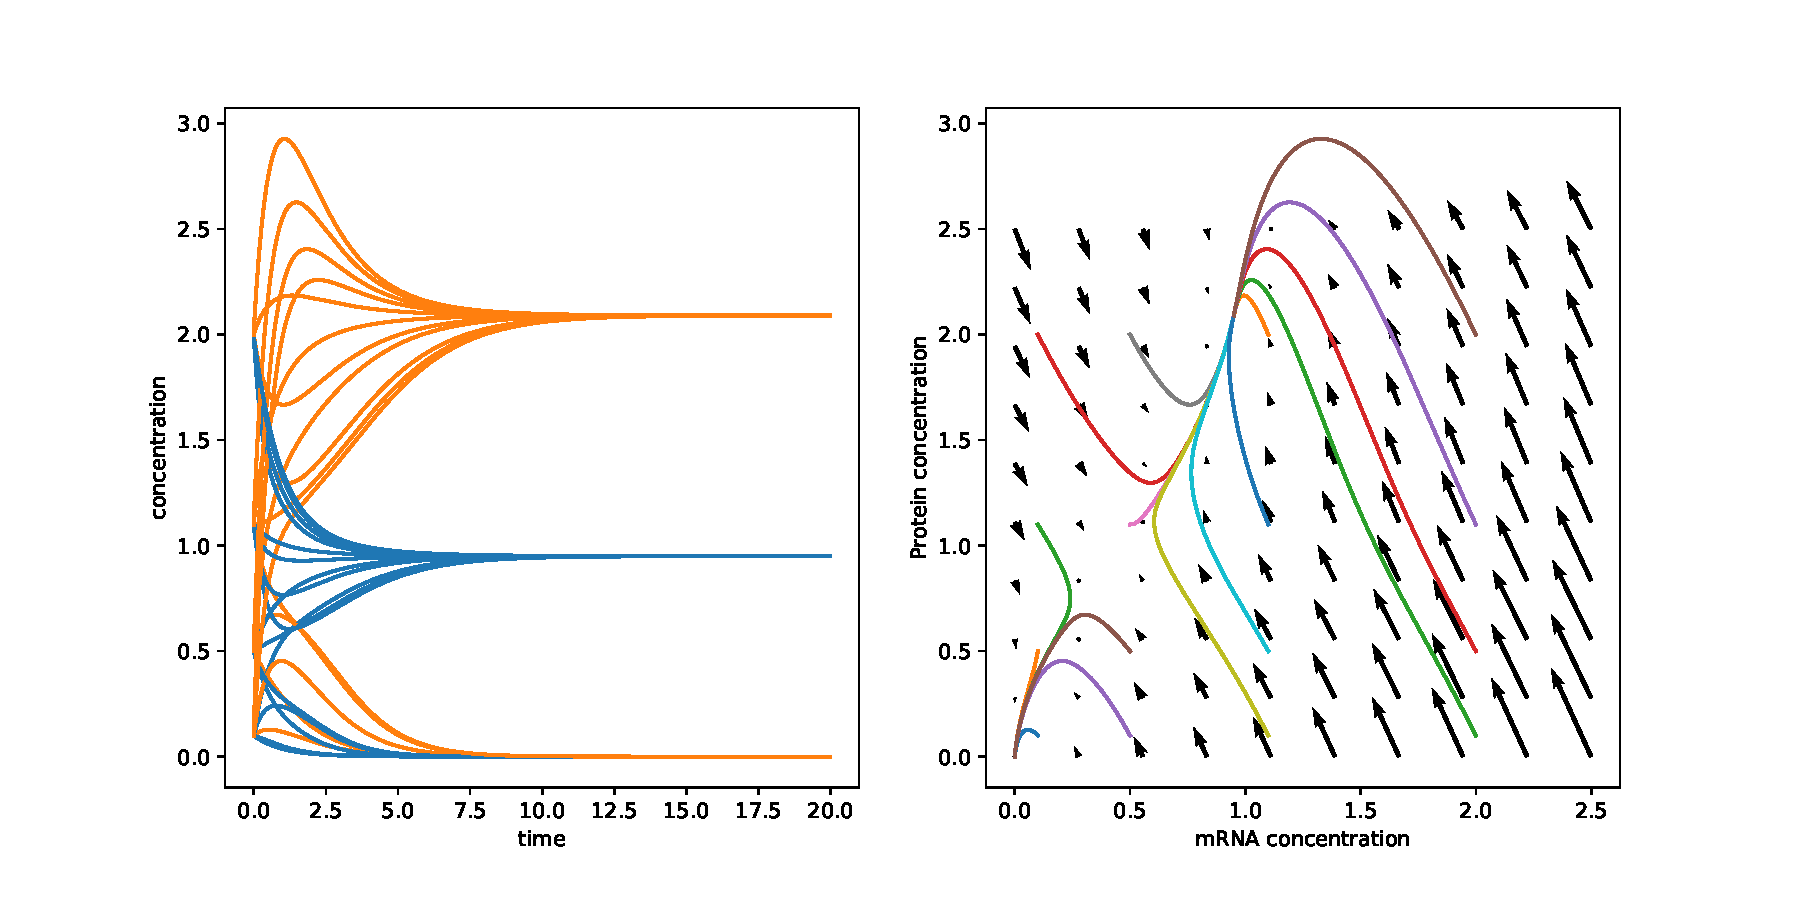
\includegraphics[width=\textwidth]{two_stable_fixed_point}
	\caption{An auto-activator with sufficiently strong cooperativity is bistable. Depending on the initial condition, the system flows towards an ``on'' or ``off'' state}
	\label{fig:bistable}
\end{figure}


\subsection*{Self repression}
Above, we considered the case of a gene product activating its own transcription and activation was modeled as Hill-function.
Repression works analogously, but the gene is transcribed with the repressor site is unbound and silent whenever a repressor is bound.
So instead of being proportional to $X^n/(K+x_2^n)$, transcription is now proportional to
\begin{equation}
	1-\frac{x_2^n}{K+x_2^n}=\frac{K}{K+x_2^n}
\end{equation}
The differential equations describing the dynamics are therefore
\begin{eqnarray}
	\label{eq:repressor}
	\frac{dx_1}{dt} &= \alpha\frac{K}{K+x_2^n} - \beta x_1 \\
	\frac{dx_2}{dt} &= \gamma x_1 - \delta x_2
\end{eqnarray}
This system has only one stable fixed point when repression and production are in balance.
Fig.~\ref{fig:repressor} show the dynamics of such a system.
Such auto-repressor systems are well suited to maintain the concentration of a species at a particular value: They work essentially like thermostats on a radiator.

Systems with negative feedback have a tendency to oscillate.
The example in Fig.~\ref{fig:repressor}, however, doesn't yet show autonomous oscillations.
To construct a true oscillator, one either needs an additional component or a stronger non-linearly/cooperativity.

\begin{figure}[tb]
	\centering
	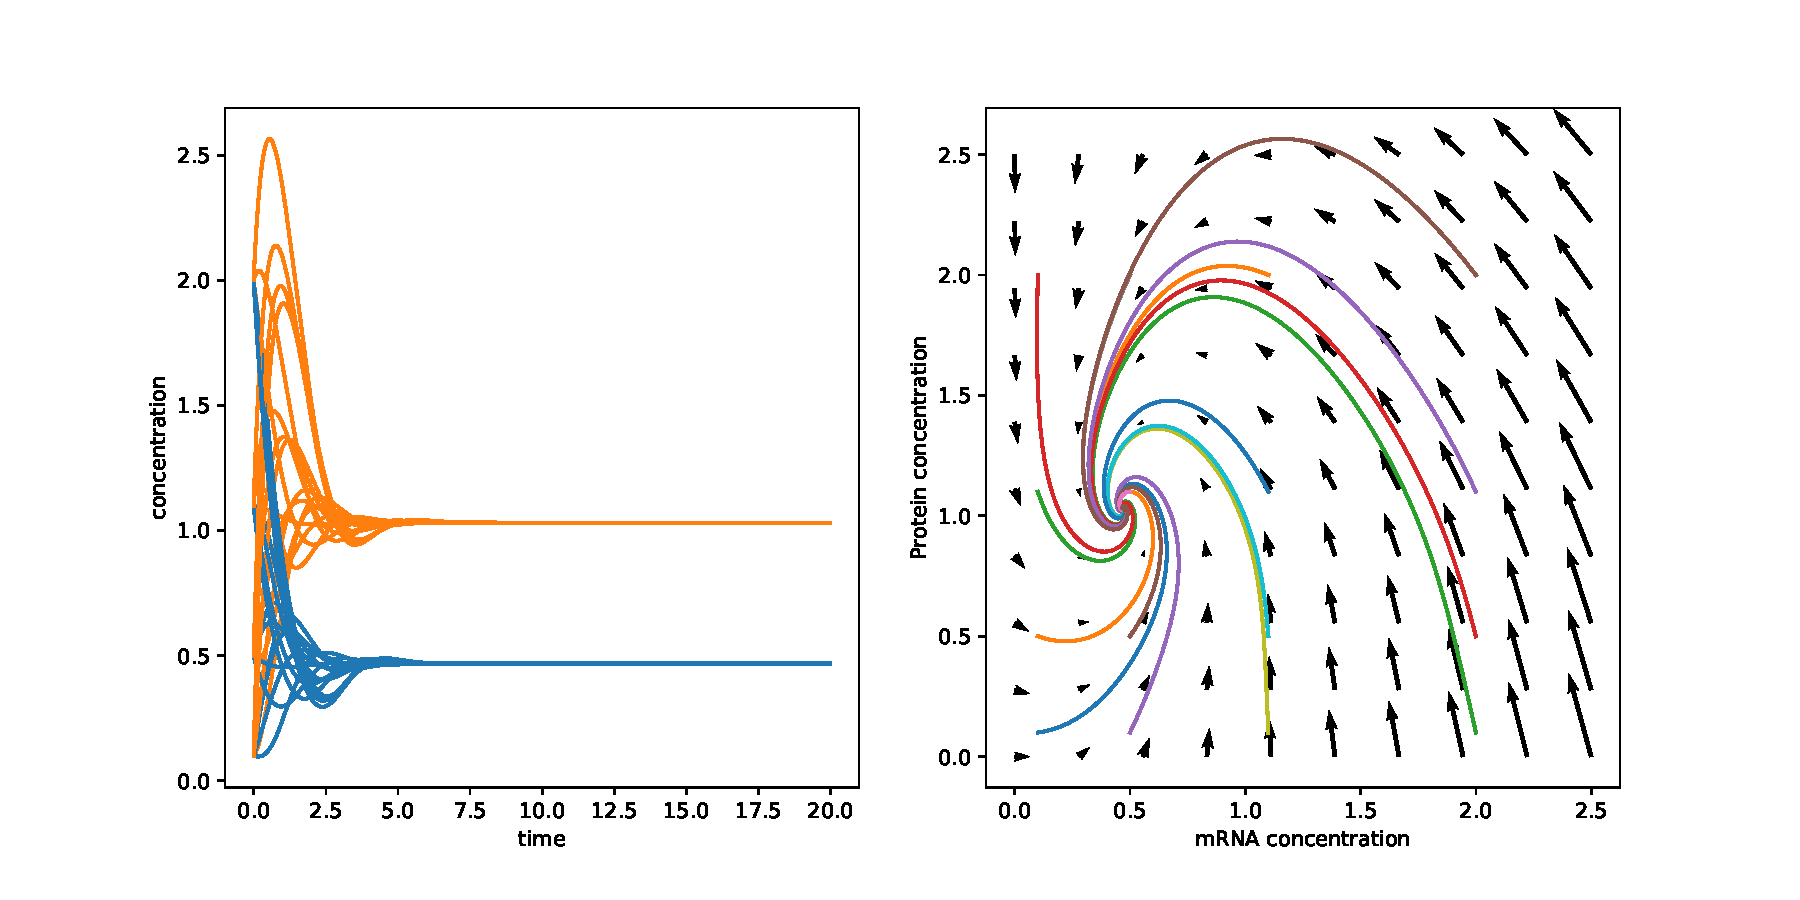
\includegraphics[width=\textwidth]{spiral_fixed_point.pdf}
	\caption{Dynamics of an auto-repressor. In this example, $\gamma=2.2$, $\delta=1$, and $n=4$.}
	\label{fig:repressor}
\end{figure}

\subsection*{Stochasticity in gene expression}
Fig.~\ref{fig:TF_abundance} shows that many TFs are present in small numbers in the cell.
As a result, the degradation or production of one TF molecule can make a substantial difference to the dynamics.
Since all molecular process are stochastic, we expect that expression of many genes and the levels of the corresponding proteins to fluctuate.

To model stochastic gene expression dynamics, one re-interprets the concentration variables as molecule numbers and the different terms in the ODEs as rates of Poisson processes.
After replacing $x$ by a discrete particle number $n$ and appropriate rescaling of the rate constants (we changed units from concentrations to particle numbers), the different terms can be interpreted as \emph{probability of a reaction per unit time}.
Given the degradation term $\delta n$, for example, the probability that $m$ particles were degraded in time interval $\Delta t$ is Poisson distributed with mean $\Delta t \delta n$.
The particle numbers can then be updated in small time steps similar to the forward Euler scheme used for deterministic ODEs in the lecture.
Note, however, that stochastic models of gene expressions are an active field of research with many sophisticated techniques to make such simulations accurate and fast.

